\section{gyakorlat (2025. október 8.)}
\subsection*{Oszd meg és uralkodj algoritmusok}
\subsubsection*{Geometria}
Adott $n$ pont a síkon. Határozzuk meg
\begin{enumerate}
    \item a két legközelebbit
    \item a két legtávolabbit.
\end{enumerate}

Kicsit távolabbról indulunk.

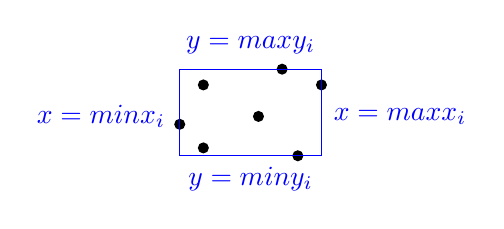
\begin{tikzpicture}
\fill (0, 0) circle(2pt);
\fill (0.3, 0.5) circle(2pt);
\fill (0.3, -0.3) circle(2pt);
\fill (1, 0.1) circle(2pt);
\fill (1.3, 0.7) circle(2pt);
\fill (1.5, -0.4) circle(2pt);
\fill (1.8, 0.5) circle(2pt);
\draw[blue] (0, -0.4) -- (0, 0.7);
\draw[blue] (0, -0.4) -- (1.8, -0.4);
\draw[blue] (1.8, 0.7) -- (1.8, -0.4);
\draw[blue] (0, 0.7) -- (1.8, 0.7);
\node at (-1, 0.1) {\color{blue}{$x = min x_i$}};
\node at (2.8, 0.1) {\color{blue}{$x = max x_i$}};
\node at (0.9, -0.7) {\color{blue}{$y = min y_i$}};
\node at (0.9, 1) {\color{blue}{$y = max y_i$}};

\end{tikzpicture}

$(x_1, y_1), (x_2, y_2), \cdots, (x_n, y_n)$ a pontok.
\setulcolor{blue}
Határozzuk meg a legkisebb olyan \ul{téglalapot} amelynek oldalai párhuzamosak a koordinátatengelyekkel és az összes pontot tartalmazza.
\setulcolor{black}

Két min és két max számolás $\rightarrow 4n-4$ összehasonlítás.
Lehet kevesebbel is?
Egyszerre $min x_i$ és $max x_i$, illetve $min y_i$ és $max y_i$?
Lássuk a $min x_i$ és $max x_i$ esetet:

$\underbrace{x_1, x_2}, \underbrace{x_3, x_4}, \underbrace{x_5, x_6}, \cdots, x_{n-2}, \underbrace{x_{n-1}, x_n}$

Az egyszerűség kedvéért tegyük fel, hogy az értékek páronként különbözőek.

Ha $x_1 < x_2$, akkor $x_1 \neq max x_i$ és $x_2 \neq min x_i \Rightarrow \left[\frac{n}{2}\right]$ összehasonlítással a feladat visszavezethető $\left\lceil\frac{n}{2}\right\rceil$ szám közül a maximum és a minimum meghatározására.
Ezzel az összehasonlítások számát $\left[\frac{n}{2}\right]$-vel tudtuk csökkenteni.
Igazából nem számít, ha az elemek között vannak megegyezőek.

Legkisebb téglalap $\rightarrow$ legkisebb sokszög (amely az összes pontot tartalmazza).

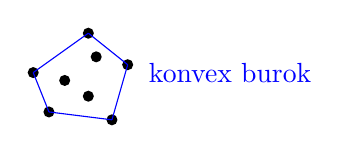
\begin{tikzpicture}
\fill (0, 0) circle(2pt);
\fill (0.2, -0.5) circle(2pt);
\fill (1, -0.6) circle(2pt);
\fill (1.2, 0.1) circle(2pt);
\fill (0.7, 0.5) circle(2pt);
\draw[blue](0, 0) -- (0.2, -0.5);
\draw[blue](0.2, -0.5) -- (1, -0.6);
\draw[blue](1, -0.6) -- (1.2, 0.1);
\draw[blue](1.2, 0.1) -- (0.7, 0.5);
\draw[blue](0.7, 0.5) -- (0, 0);
\fill (0.4, -0.1) circle(2pt);
\fill (0.7, -0.3) circle(2pt);
\fill (0.8, 0.2) circle(2pt);
\node at (2.5, 0) {\color{blue}{konvex burok}};
\end{tikzpicture}

Nem nehéz belátni, hogy a két legtávolabbi pont a konvex burok két csúcsa.

\setulcolor{blue}
Az első lépés a két legtávolabbi pont meghatározásához a \ul{konvex burok meghatározása}.
\setulcolor{black}

$(x_1, y_1), (x_2, y_2), \cdots, (x_n, y_n) \rightarrow$ a konvex burok csúcsainak felsorolása a konvex burkon az óramutató járása szerint.

Milyen "bonyolult" a konvex burok meghatározása?
Legalább annyira, mint a rendezés.

$(x_1, x_1^2), (x_2, x_2^2), \cdots, (x_n, x_n^2)$ bemenethez:

\begin{tikzpicture}
\begin{axis}[
    axis lines=middle,
    ymin=-2, ymax=8,
    xmin=-1, xmax=4,
    restrict x to domain=-0.1:2.5,
    xticklabel=\empty,
    yticklabel=\empty,
    xtick=\empty,
    ytick=\empty
]
    \addplot[mark=none] {pow(x,2)} node[right]{$y=x^2$};
\end{axis}

\node[orange] at (2, 0.9) {$x_{i_1}$};
\node[orange] at (2.5, 0.9) {$x_{i_2}$};
\node[orange] at (3, 0.9) {$x_{i_3}$};
\node[orange] at (4, 0.9) {$\cdots$};

\fill[orange] (2, 1.25) circle(2pt);
\fill[orange] (2.5, 1.52) circle(2pt);
\fill[orange] (3, 1.95) circle(2pt);
\fill[orange] (3.5, 2.52) circle(2pt);
\fill[orange] (4, 3.25) circle(2pt);
\fill[orange] (4.5, 4.12) circle(2pt);

\draw[orange] (2, 1.15) -- (2, 1.25);
\draw[orange] (2.5, 1.15) -- (2.5, 1.52);
\draw[orange] (3, 1.15) -- (3, 1.95);
\draw[orange] (3.5, 1.15) -- (3.5, 2.52);
\draw[orange] (4, 1.15) -- (4, 3.25);
\draw[orange] (4.5, 1.15) -- (4.5, 4.12);

\draw[red] (2, 1.25) -- (4.5, 4.12);
\node[red] at (3, 2.9) {\lcirclearrowright};
\end{tikzpicture}

\clearpage
Egy konvex burok algoritmus rendezi is az $x_1, x_2, \cdots, x_n$ számokat (csökkenően).
$\mathcal{O}(n \log n)$ költségűek a "jó" konvex burok algoritmusok.
Több ilyen is van, oszd meg és uralkodj is:

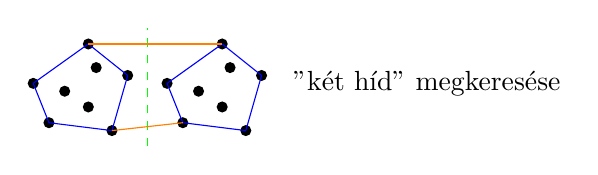
\begin{tikzpicture}
\fill (0, 0) circle(2pt);
\fill (0.2, -0.5) circle(2pt);
\fill (1, -0.6) circle(2pt);
\fill (1.2, 0.1) circle(2pt);
\fill (0.7, 0.5) circle(2pt);
\draw[blue](0, 0) -- (0.2, -0.5);
\draw[blue](0.2, -0.5) -- (1, -0.6);
\draw[blue](1, -0.6) -- (1.2, 0.1);
\draw[blue](1.2, 0.1) -- (0.7, 0.5);
\draw[blue](0.7, 0.5) -- (0, 0);
\fill (0.4, -0.1) circle(2pt);
\fill (0.7, -0.3) circle(2pt);
\fill (0.8, 0.2) circle(2pt);

\draw[green, dashed] (1.45, -0.8) -- (1.45, 0.7);

\fill (1.7, 0) circle(2pt);
\fill (1.9, -0.5) circle(2pt);
\fill (2.7, -0.6) circle(2pt);
\fill (2.9, 0.1) circle(2pt);
\fill (2.4, 0.5) circle(2pt);
\draw[blue](1.7, 0) -- (1.9, -0.5);
\draw[blue](1.9, -0.5) -- (2.7, -0.6);
\draw[blue](2.7, -0.6) -- (2.9, 0.1);
\draw[blue](2.9, 0.1) -- (2.4, 0.5);
\draw[blue](2.4, 0.5) -- (1.7, 0);
\fill (2.1, -0.1) circle(2pt);
\fill (2.4, -0.3) circle(2pt);
\fill (2.5, 0.2) circle(2pt);

\draw[orange] (0.7, 0.5) -- (2.4, 0.5);
\draw[orange] (1, -0.6) -- (1.9, -0.5);
\node at (5, 0){"két híd" megkeresése};
\end{tikzpicture}

\begin{enumerate}
    \item két feleakkora feladat
    \item rekurzívan megoldjuk a részfeladatokat
    \item "egyesítjük" a két konvex burkot (két híd)
\end{enumerate}

Ezek után a két legtávolabbi csúcs a konvex burkon (nem oszd meg és uralkodj algoritmus):

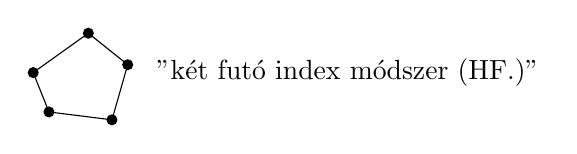
\begin{tikzpicture}
\fill (0, 0) circle(2pt);
\fill (0.2, -0.5) circle(2pt);
\fill (1, -0.6) circle(2pt);
\fill (1.2, 0.1) circle(2pt);
\fill (0.7, 0.5) circle(2pt);
\draw(0, 0) -- (0.2, -0.5);
\draw(0.2, -0.5) -- (1, -0.6);
\draw(1, -0.6) -- (1.2, 0.1);
\draw(1.2, 0.1) -- (0.7, 0.5);
\draw(0.7, 0.5) -- (0, 0);
\node at (4, 0){"két futó index módszer (HF.)"};
\end{tikzpicture}

\subsubsection*{Minimális távolság}

\textbf{Oszd meg és uralkodj algoritmus}

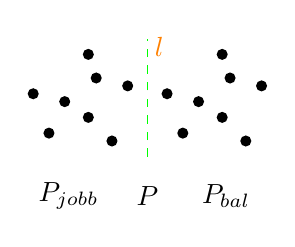
\begin{tikzpicture}
\fill (0, 0) circle(2pt);
\fill (0.2, -0.5) circle(2pt);
\fill (1, -0.6) circle(2pt);
\fill (1.2, 0.1) circle(2pt);
\fill (0.7, 0.5) circle(2pt);
\fill (0.4, -0.1) circle(2pt);
\fill (0.7, -0.3) circle(2pt);
\fill (0.8, 0.2) circle(2pt);

\fill (1.7, 0) circle(2pt);
\fill (1.9, -0.5) circle(2pt);
\fill (2.7, -0.6) circle(2pt);
\fill (2.9, 0.1) circle(2pt);
\fill (2.4, 0.5) circle(2pt);
\fill (2.1, -0.1) circle(2pt);
\fill (2.4, -0.3) circle(2pt);
\fill (2.5, 0.2) circle(2pt);

\draw[green, dashed] (1.45, -0.8) -- (1.45, 0.7);

\node at (1.6, 0.6){\color{orange} $l$};
\node at (1.45, -1.3){$P$};
\node at (2.45, -1.3){$P_{bal}$};
\node at (0.45, -1.3){$P_{jobb}$};
\end{tikzpicture}

\begin{enumerate}
    \item két feleakkora feladatra bontás $\rightarrow P_{bal}, P_{jobb}$
    \item rekurzívan meghatározzuk a minimális távolságot $P_{bal}$-ban és $P_{jobb}$-ban:
    \begin{itemize}
        \item $P_{bal} \rightarrow \delta_{bal}$
        \item $P_{jobb} \rightarrow \delta_{jobb}$
    \end{itemize}
    \item minimális távolság meghatározása
\end{enumerate}

A minimális távolság vagy baloldalon vagy jobboldalon van, vagy keresztezi az $l$ felező egyenest.

A harmadik esetben $l$-től nem túl messze lévő pontokra elég szorítkozni.\\
Legyen $\delta = min(\delta_{bal}, \delta_{jobb})$.

\begin{tikzpicture}
\draw (0, 0) -- (0, 4);
\draw (2, 0) -- (2, 4);
\draw[dashed] (1, 0) -- (1, 4);

\node at (1.3, 3.6){$l$};

\draw[->] (0, 0.5) -- (1, 0.5);
\draw[->] (1, 0.5) -- (0, 0.5);
\draw[->] (1, 0.5) -- (2, 0.5);
\draw[->] (2, 0.5) -- (1, 0.5);

\node at (0.5, 0.25){$\delta$};
\node at (1.5, 0.25){$\delta$};
\end{tikzpicture}

Ebben a $\delta$ sugarú sávban kell a két pontnak lenni, amelyek a min távolságot minimalizálják.

\clearpage
Itt van még valami, amit érdemes észrevenni.
Tekintsük a sávbeli pontokat az $y$ koordinátájuk szerint monoton növekvően rendezetten.

\begin{tikzpicture}
\draw (0, 0) -- (0, 4);
\draw (2, 0) -- (2, 4);
\draw (1, 0) -- (1, 4);

\draw[->] (0, 0.5) -- (1, 0.5);
\draw[->] (1, 0.5) -- (0, 0.5);
\draw[->] (1, 0.5) -- (2, 0.5);
\draw[->] (2, 0.5) -- (1, 0.5);

\node at (0.5, 0.25){$\delta$};
\node at (1.5, 0.25){$\delta$};

\draw[blue] (0, 1.5) -- (2, 1.5);
\draw[blue] (0, 2.5) -- (2, 2.5);
\draw[blue, ->] (-0.25, 1.5) -- (-0.25, 2.5);
\draw[blue, ->] (-0.25, 2.5) -- (-0.25, 1.5);
\node[blue] at (-0.5, 2){$\delta$};
\fill (0.5, 1.5) circle(2pt);
\node at (6, 1){"első pont" $\rightarrow$ hány ponttól lehet $\delta$-nál közelebb?};
\draw[-Latex] (2.2, 1) -- (0.5, 1.5);
\end{tikzpicture}

Minden ilyen pont szükségképpen ebben a téglalapban van:

\begin{tikzpicture}
\draw[blue] (0, 0) -- (4, 0);
\draw[blue] (0, 2) -- (4, 2);
\draw (2, 0) -- (2, 2);
\draw (0, 0) -- (0, 2);
\draw (4, 0) -- (4, 2);
\draw[dashed] (0, 1) -- (4, 1);
\draw[dashed] (1, 0) -- (1, 2);
\draw[dashed] (3, 0) -- (3, 2);

\node at (-0.3, 1){$\delta$};
\node at (1, -0.3){$\delta$};
\node at (3, -0.3){$\delta$};

\fill (0.7, 0) circle(2pt);
\end{tikzpicture}

Tekintsük a fenti 8 kis négyzetet.
Mivel ezek átmérője $\frac{8}{2} \sqrt{2} = \frac{8}{\sqrt{2}} < \delta$, és az $l$ bal, illetve jobb oldalán a minimális távolság legalább $\delta$, így a 8 kis négyzet egyikében sem lehet egynél több $P$-beli pont.
Így a legalsó ponttól $\delta$-nál kisebb távolságra csak a következő 7 pont valamelyike lehet.
Felfelé haladva ez mindig igaz lesz.

Költség: $T(n) = 2T(\frac{n}{2}) + \underbrace{\mathcal{O}(n \log n)}_{\text{rendezések}} \rightarrow T(n) ( \mathcal{O}(n \log^2 n))$

$\mathcal{O}(n \log^2 n) \rightarrow \mathcal{O}(n \log n)$


Előfeldolgozás $\rightarrow$ előrendezés (x és y koordináták szerint is) $\rightarrow$ rekurzív hívásokban már csak kiválogatás

$T(n) = 2T(\frac{n}{2}) + \mathcal{O}(n) \rightarrow T(n) = \mathcal{O}(n \log n)$